% This ensures VS Code compiles the main file even when you're editing a chapter.
% !TeX root = ../main.tex

\chapter{Implementation}
\label{cap:impl}

The following sections will detail how the chosen modules were assembled, connected,
what kind of algorithms were programmed in the two subsystems and what kind of tests
were executed in order to evaluate the pod system's performance.

\section{The prototype}

A detailed connection diagram of the whole test device can be seen in
Figure~\ref{fig:5ckt}.

\begin{figure}[ht]
  \centering
  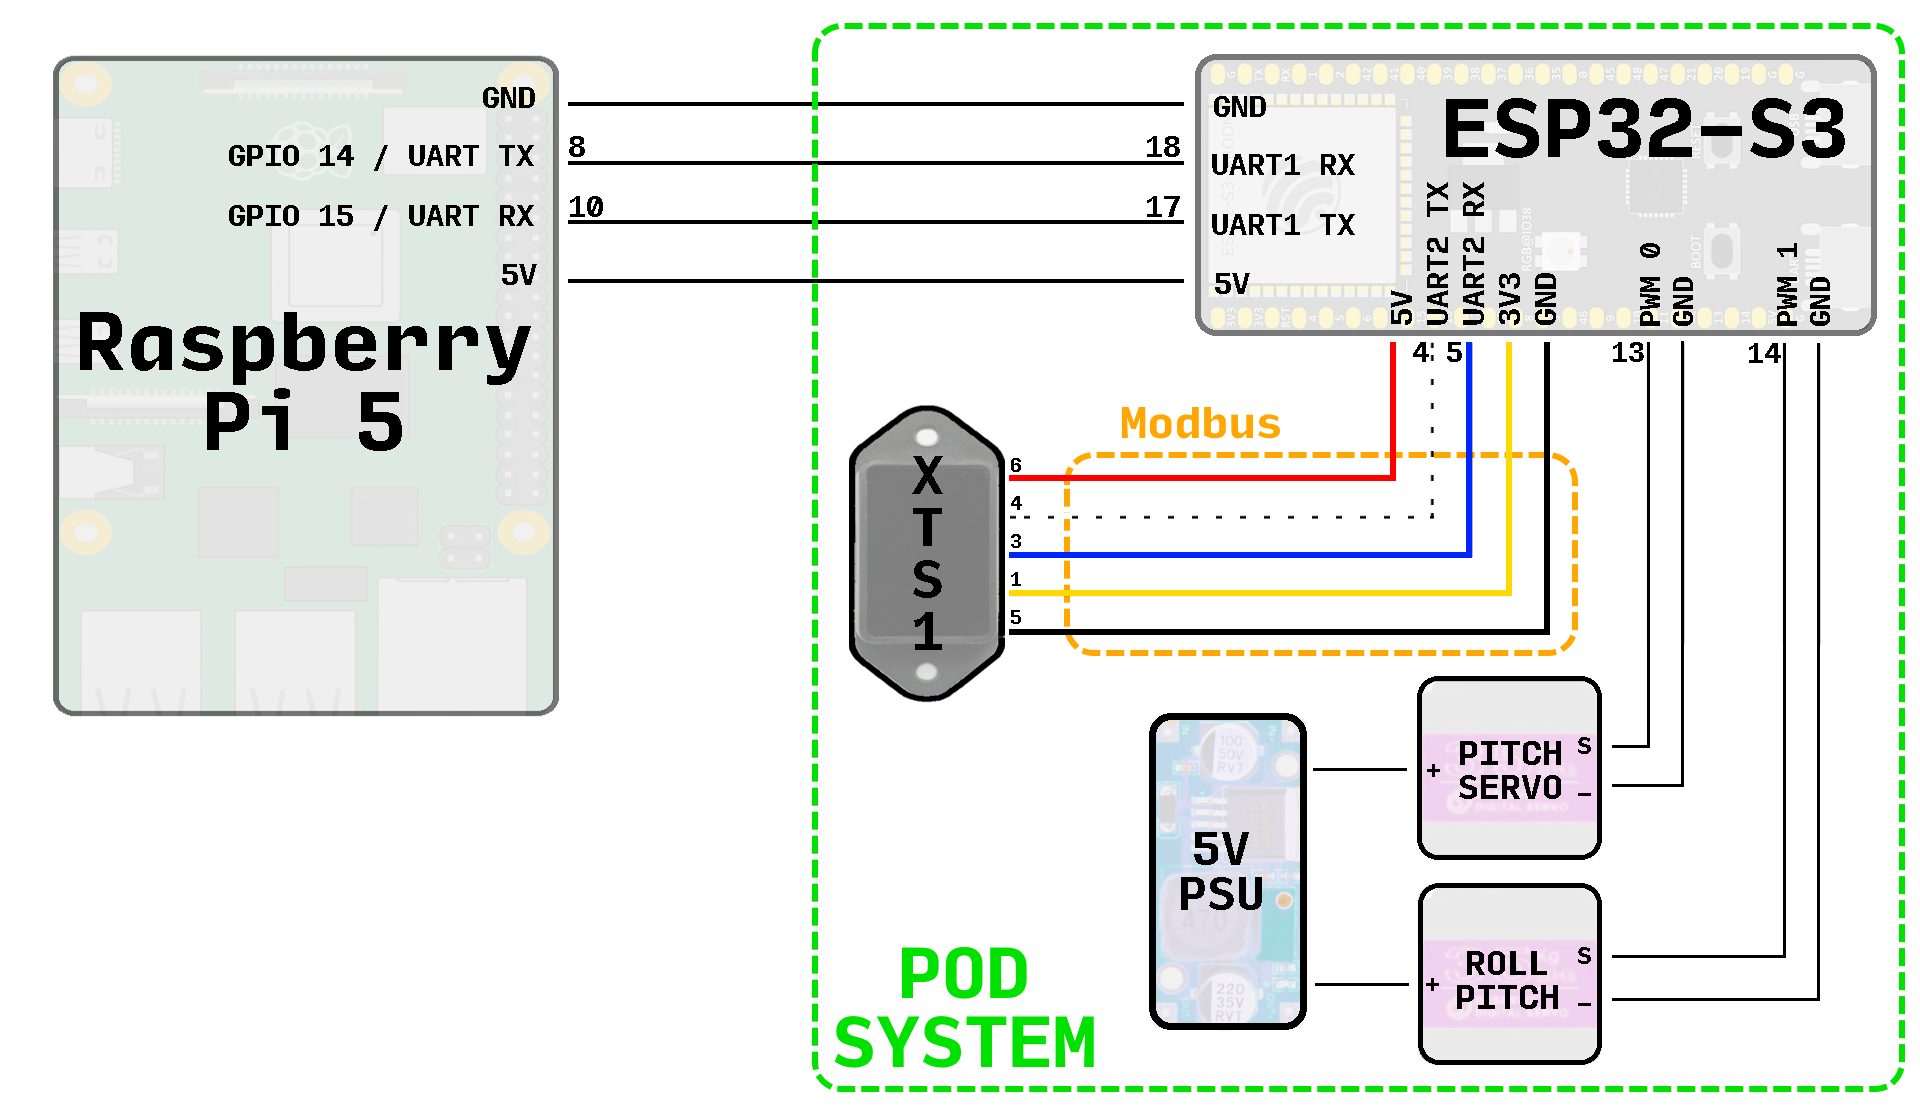
\includegraphics[width=1\textwidth]{5/img1}
  \caption{Connection diagram of the whole project}
  \label{fig:5ckt}
\end{figure}

Both communication buses from the ESP32-S3 to the Raspberry Pi 5 and the XT-S1
use \gls{uart} communication. For the XT-S1 sensor, Modbus \cite{modbus}
is implemented on top of \gls{uart}, for a safe, reliable connection.
The protocol used to set the servos in position is simple \gls{pwm}.
The 5V rail from the Raspberry Pi is used to supply power to the ESP32-S3 and the
XT-S1 sensor.
A separate 5V \gls{psu} unit is used for the servos alone, as they draw high
currents during startup and when moving the main axis, which would not be supported
by the 5V supply from the Raspberry Pi.

\subsection{Prototype's evolution}

The prototype 3D case was designed over many different iterations.
The final version of the case can be seen by the end of Chapter~\ref{cap:prop}.
The specific \gls{pn} of the servo was selected after the most common
TowerPro SG90 (9g Servo) showed unacceptable backlash and slack.

The Raspberry pi 5 also took some efforts to operate reliably.
Without officialy recommended peripherals, the \gls{sbc} showed problems with:

\begin{itemize}
  \item Power supply instability.
  \item Thermal management.\end{itemize}

Without warning, the \gls{sbc} would stop properly working or even shut down.
The Raspberry Pi operated without any issues only when equipped with the official
heat sink and \gls{psu}.

\subsection{Raspberry Pi's test UI}

 W I P

\section{The tests}

The following sections will exaplain in details the three tests:

\begin{itemize}
  \item Static single-point test.
  \item Static multi-point test.
  \item Dynamic test.
\end{itemize}

To test a device that calculates distances based on a laser rangefinder
mounted on a gimbal, first
it is important to assess how accurate and precise the laser rangefinder is. For
that, a static single-point test can be executed, measuring the distance to a
known, easy to acquire target. After the rangefinder is tested, the gimbal
must be tested as well. A static multi-point test can check if the angles
requested by the drone system are being correctly set by the motors. The target
can be any planar surface. Multiple points are requested as targets and any
error in this test will propagate into the reconstructed 3D geometry.
With both the rangefinder and
gimbal tested, the system must be tested against a moving target. A dynamic test
to measure the angular performance of the system can assess if the system can
keep track and measurement of a target moving within the system's limits.

\subsection{Static single-point test}

The single-point static test characterizes the accuracy and precision of the
range estimation module under controlled, time-invariant conditions. A flat
target of known reflectance is mounted perpendicular to the optical axis of the
sensor on a rigid fixture, and its distance is established by an independent
reference instrument of substantially lower uncertainty than the device under
test (DUT), such as a calibrated laser distance meter or a precision linear
stage with a traceable encoder. The test is repeated at $K$ nominal distances
$d_{\mathrm{ref},k}$, $k=1,\dots,K$, spanning the specified operating range of
the module. At each distance, $N$ consecutive measurements $\hat{d}_{k,i}$ are
acquired after a thermal stabilization period of X\,min, with
ambient illumination, target reflectance, and temperature recorded throughout.

Following the terminology of ISO~5725 \cite{iso5725}, accuracy is decomposed into
\emph{trueness} and \emph{precision}. For each distance, the sample mean and
the bias are computed as
\begin{equation}
  \bar{d}_k = \frac{1}{N}\sum_{i=1}^{N}\hat{d}_{k,i}, \qquad
  b_k = \bar{d}_k - d_{\mathrm{ref},k},
\end{equation}
while precision is quantified by the sample standard deviation
\begin{equation}
  \sigma_k = \sqrt{\frac{1}{N-1}\sum_{i=1}^{N}\left(\hat{d}_{k,i}-\bar{d}_k\right)^2}.
\end{equation}
The overall error is summarized by the root-mean-square error,
\begin{equation}
  \mathrm{RMSE}_k = \sqrt{b_k^2 + \sigma_k^2 \,\frac{N-1}{N}},
\end{equation}
which combines systematic and random contributions. To expose range-dependent
behavior, the bias $b_k$ is regressed against $d_{\mathrm{ref},k}$ to separate
a constant offset from a scale (gain) error, and $\sigma_k$ is examined as a
function of distance and signal amplitude. Measurement uncertainty is reported
according to the Guide to the Expression of Uncertainty in Measurement
(JCGM~100:2008) \cite{jcgm100}, combining the DUT repeatability with the reference
instrument uncertainty and the target alignment error.

An important point in this test is that, even though \emph{trueness} can be adjusted
by a calibration process in firmware after the tests, to improve accuracy,
the \emph{precision}
of the overall system is mainly determined by the precision of the sensor, which in
this system's case, comes pre-calibrated from the manufacturer. The standard
deviation of the distances measured will be mainly a product of the chosen sensor,
luminous noise at the target and distance, as the chosen sensor presents optimal
ranges for the measurements, and becomes less accurate when measuring very close
distances. So in the end, the overall error can be minimized by compensating any
error in the trueness of the measurements.

\subsubsection{Servos}

The servos, just as the laser rangefinder, will need to have their trueness
calibrated. Just as with the rangefinder, the precision is a product of the the
manufacturer specifications, which can be found in the part's datasheet.
What can be done regarding the servos is using a bias value to compensate for
any drift on the control circuit and any imprecision on the 3D parts that, with
the servo, compose the gimbal.

\subsection{Static multi-point test}

The multipoint test evaluates the three-dimensional performance of the module
over its field of view (FoV). A planar target of known flatness, larger than
the footprint of the FoV at the test distance, is positioned at a nominal
distance $d_0$ and its pose relative to the sensor frame is established with
the reference instrument. For a sensor that outputs $M$ measurement points
(zones or pixels), each point is converted to Cartesian coordinates
$\mathbf{p}_j=(x_j,y_j,z_j)^\top$ using the sensor's intrinsic angular
calibration, with $N$ frames averaged or retained per point as appropriate.

The reference plane is described by $\mathbf{n}^\top\mathbf{p}=\rho$, with unit
normal $\mathbf{n}$ and offset $\rho$. The measured points are fitted to a plane
by total least squares, with the normal obtained as the singular vector
associated with the smallest singular value of the centered point matrix. The
point-to-plane residuals are
\begin{equation}
  r_j = \mathbf{n}^\top\mathbf{p}_j - \rho, \qquad
  \mathrm{RMS}_{\mathrm{plane}} = \sqrt{\frac{1}{M}\sum_{j=1}^{M} r_j^2},
\end{equation}
and quantify the overall three-dimensional consistency of the measurement,
including per-zone bias, lens distortion residuals, and inter-zone crosstalk.
In addition, the angular deviation between the fitted and reference normals,
\begin{equation}
  \Delta\theta = \arccos\left(\mathbf{n}_{\mathrm{fit}}^\top \mathbf{n}_{\mathrm{ref}}\right),
\end{equation}
and the per-zone range error with respect to the reference plane are reported,
the latter as a spatial error map revealing systematic patterns such as
radial bias or edge-of-FoV degradation. The test is repeated for several
distances and target tilt angles to assess the dependence of the error on
incidence angle, and, where relevant, for several surface reflectances.

\section{Dynamic test}

The dynamic test assesses the ability of the module to follow a moving target
and characterizes its temporal behavior, which static tests cannot capture. The
target is mounted on a motorized linear stage whose position $d_{\mathrm{ref}}(t)$
is recorded by an encoder (or other reference instrument) with a sampling rate
well above that of the DUT. The reference and DUT data streams are
synchronized through a common trigger or hardware timestamp, and residual clock
offset is estimated and removed in post-processing. Three motion profiles are
considered: (i)~constant-velocity ramps at several speeds $v$, to evaluate
velocity-dependent error; (ii)~a step displacement, to evaluate the transient
response and settling time; and (iii)~sinusoidal motion at increasing
frequencies, to estimate the effective measurement bandwidth.

The tracking error is defined as
\begin{equation}
  e(t_i) = \hat{d}(t_i) - d_{\mathrm{ref}}(t_i),
\end{equation}
from which the RMSE, the maximum absolute error, and the error as a function of
target velocity are computed. The effective latency $\tau$ of the module is
estimated as the lag that maximizes the cross-correlation between the measured
and reference signals,
\begin{equation}
  \tau = \arg\max_{\delta}\sum_i \hat{d}(t_i)\,d_{\mathrm{ref}}(t_i-\delta),
\end{equation}
and the error is subsequently reported both with and without latency
compensation, separating the delay contribution from the intrinsic measurement
error. Further metrics include the effective output rate, the percentage of
invalid or dropped samples, the step-response settling time to within
X\,\% of the final value, and the $-3\,\mathrm{dB}$ bandwidth
obtained from the sinusoidal sweep. Together, these metrics determine the
maximum target speed and dynamics for which the module satisfies the
accuracy requirements of the intended application.
